\documentclass[tikz]{standalone}

% based on https://upload.wikimedia.org/wikipedia/commons/8/8b/Sidereal_day_%28prograde%29.svg

\begin{document}
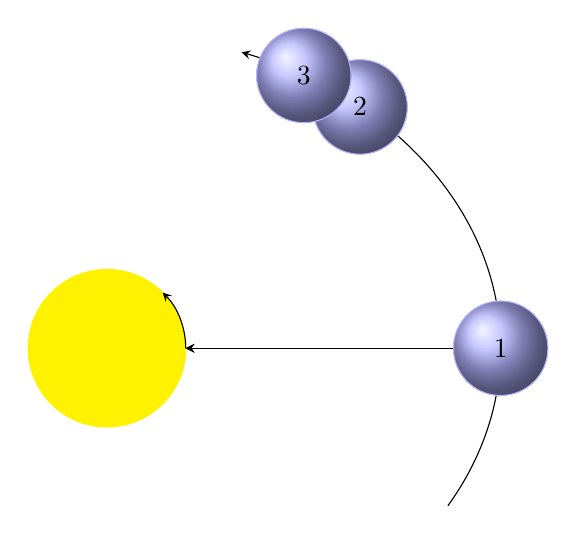
\begin{tikzpicture}[scale=2]

  % Draw the Sun
  \draw[fill=yellow, draw=yellow] (0,0) circle (0.5);

  % Define the angle of rotation of the Earth
  \pgfmathsetmacro\angle{45}

  % Define the center and radii of the ellipse
  \def\cx{0}
  \def\cy{0}
  \def\rx{2.5}
  \def\ry{2}

  % Define the start and end angles of the arc
  \def\startangle{-30}
  \def\endangle{70}

  % Draw the arc
  \draw[-stealth] (\startangle:\rx cm and \ry cm) arc (\startangle:\endangle:\rx cm and \ry cm);

  % Define the positions of the planets
  \def\pA{0}
  \def\pB{50}
  \def\pC{60}

  % Calculate the coordinates of the planets
  \coordinate (A) at ({\cx + \rx*cos(\pA)}, {\cy + \ry*sin(\pA)});
  \coordinate (B) at ({\cx + \rx*cos(\pB)}, {\cy + \ry*sin(\pB)});
  \coordinate (C) at ({\cx + \rx*cos(\pC)}, {\cy + \ry*sin(\pC)});

  \def\color{blue!30}

  \draw[-stealth] (A) -- (0.5,0);
  \draw[-stealth] (A) -- (0.5,0);


  % Draw the planets as circles
  \filldraw[ball color=\color,draw=\color] (A) circle (0.3) node {1};
  \filldraw[ball color=\color,draw=\color] (B) circle (0.3) node {2};
  \filldraw[ball color=\color,draw=\color] (C) circle (0.3) node {3};

  % Draw the angle of rotation of the Earth
  \draw[-stealth] (0,0) ++(0.5,0) arc (0:\angle:0.5);

\end{tikzpicture}

\end{document}
